\begin{figure}[t]
\centering
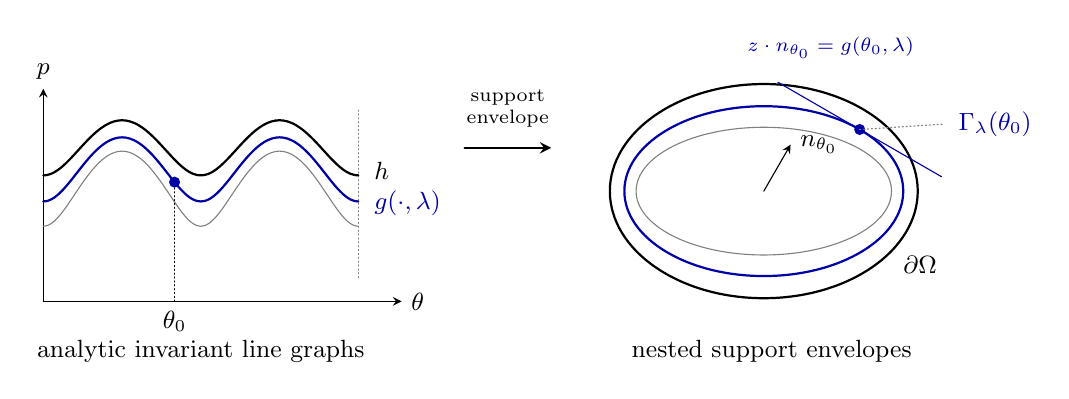
\begin{tikzpicture}[font=\small,>=stealth,line cap=round]
  \pgfmathsetmacro{\selectedsupport}{sqrt(4.34*cos(60)^2+1.61*sin(60)^2)}
  \pgfmathsetmacro{\contactx}{.85*4.34*cos(60)/\selectedsupport}
  \pgfmathsetmacro{\contacty}{.85*1.61*sin(60)/\selectedsupport}
  \begin{scope}
    \draw[->] (0,0)--(4.55,0) node[right] {$\theta$};
    \draw[->] (0,0)--(0,2.7) node[above] {$p$};
    \draw[densely dotted,gray] (4,.3)--(4,2.45);
    \draw[thick,domain=-90:270,samples=81,smooth,variable=\a]
      plot ({(\a+90)/90},{sqrt(5.29*cos(\a)^2+2.56*sin(\a)^2)});
    \draw[blue!65!black,thick,domain=-90:270,samples=81,smooth,variable=\a]
      plot ({(\a+90)/90},{sqrt(4.34*cos(\a)^2+1.61*sin(\a)^2)});
    \draw[gray,domain=-90:270,samples=81,smooth,variable=\a]
      plot ({(\a+90)/90},{sqrt(3.64*cos(\a)^2+.91*sin(\a)^2)});
    \node[anchor=west] at (4.08,1.66) {$h$};
    \node[anchor=west,blue!65!black] at (4.08,1.25) {$g(\cdot,\lambda)$};
    \draw[densely dotted] (1.6667,0)--(1.6667,\selectedsupport);
    \fill[blue!65!black] (1.6667,\selectedsupport) circle (2pt);
    \node[below] at (1.6667,0) {$\theta_0$};
    \node at (2,-.63) {analytic invariant line graphs};
  \end{scope}
  \draw[->,thick] (5.35,1.95)--(6.45,1.95);
  \node[align=center,font=\scriptsize] at (5.9,2.45) {support\\envelope};
  \begin{scope}[xshift=9.15cm,yshift=1.4cm]
    \draw[thick] (0,0) ellipse [x radius=1.955,y radius=1.36];
    \draw[blue!65!black,thick] (0,0)
      ellipse [x radius=1.77076,y radius=1.07853];
    \draw[gray] (0,0) ellipse [x radius=1.62173,y radius=.81086];
    \draw[blue!65!black]
      ({\contactx-1.2*cos(150)},{\contacty-1.2*sin(150)})--
      ({\contactx+1.2*cos(150)},{\contacty+1.2*sin(150)});
    \fill[blue!65!black] (\contactx,\contacty) circle (2pt);
    \draw[gray,thin,densely dotted] (\contactx,\contacty)--(2.27,.85);
    \node[anchor=west,blue!65!black] at (2.35,.85)
      {$\Gamma_\lambda(\theta_0)$};
    \node[anchor=south,blue!65!black,font=\scriptsize] at (.85,1.56)
      {$z\cdot n_{\theta_0}=g(\theta_0,\lambda)$};
    \draw[->] (0,0)--(.34,.59) node[right] {$n_{\theta_0}$};
    \node[anchor=west] at (1.65,-.93) {$\partial\Omega$};
    \node at (.1,-2.03) {nested support envelopes};
  \end{scope}
\end{tikzpicture}
\caption{The support-envelope correspondence, drawn schematically.
The highlighted point of $p=g(\theta,\lambda)$ specifies the blue
tangent line on the right; its contact point is
$\Gamma_\lambda(\theta_0)=g n_{\theta_0}+g_\theta e_{\theta_0}$,
with $g$ and $g_\theta$ evaluated at $(\theta_0,\lambda)$.
Positive $g+g_{\theta\theta}$ makes each envelope strictly convex,
and $g_\lambda<0$ makes the family strictly nested.}
\label{fig:phase-to-caustic}
\end{figure}
